%!TEX root = thesis.tex
%% %% ***************** Results *****************


\section{Results}\label{sec:results}

We start this section by looking at
the Azure resources needed for ML training
both on common Azure environment and ML Studio.
Next we analyze the results of
different ML algorithms and pipelines.

\subsection{Azure and Azure ML Studio}\label{subsec:azure-and-azure-ml-studio}

\subsubsection*{Azure resources}
\begin{itcomment}
    what resources was needed inside Azure?

    virtual machines etc.

    Unless these were discussed in previous sections.
\end{itcomment}


Due to some restrictions in security,
all resources used for ML training
needed to be inside the same virtual network.
Azure ML Studio environment could be opened from any network,
but most of the features were unavailable
if accessing machine was outside this virtual network.
Thus,
a virtual machine had to be acquired as Azure resource
from within the same network as other resources
and ML Studio internet UI had to be opened with this machine.

%% TODO: add picture to explain this

\subsubsection*{Azure ML Studio components}
\begin{itcomment}
    clusters and data

    Memory problems
\end{itcomment}

During the initial pipeline runs
the execution came to an abrupt stop
and Azure notified about memory issues.
These problems were linked to the data amount
which had to be reduced to 600 megabytes
before any pipeline could be finished using the data.
This reduction was against the initial goal
where preferably all the data could have been used.

Considerable amount of time was used
to fix or avoid this issue
but nothing clear was found
that would explain the error received.
While working with the issue
it was also noted
that data needed more cleaning
in order to ease the preprocessing phase
as described with more detail in section~\ref{subsec:meth-data-anonymization}
Thus,
the data had to be imported from log archive
and anonymized once more.

Two choices was possible to take:
\begin{enumerate}
    \item Continue working with full data
    and try to fix the memory issue
    by consulting Azure experts
    \item  Trim the data to reduce the data size
    by declaring info-type log messages
    as unnecessary
    and working with vastly diminished data
    until the memory issue would be solved
    one way or another
\end{enumerate}

To advance the study more efficiently
it was decided to trim info-type log messages from data
hence reducing the data amount considerably.
Final data included 8.6 million log rows
which was about 10\% of the original data size.

Even with this data size,
some Azure ML components faced this memory issue
and forced us to choose such components
that were able to handle these data amounts.

%% TODO: Move some parts of the above memory problem elsewhere

In addition to the data we used to train the algorithm,
we needed to set up computing instance
in Azure ML studio.
Some predefined resource limitations
affected the computing instance choosing
and the memory issue encouraged us
to pick memory prioritized instances.
Single computing instance did not work,
but we needed to choose a computing cluster instead
to be able to run ML training pipeline.
%% TODO: Maybe what other choises were possible?



\subsection{ML training and validation}\label{subsec:ml-training-and-validation}

\begin{itcomment}
    anomaly detection

    N-Gram Feature extracting

    Some regression algorithm to predict event count.
    Poisson only for poisson distributed data, probably not usable here

    two-class classification
    support vector machine etc

    random forest regression is probably best based on the initial results
\end{itcomment}

preformatting data! \\
\begin{enumerate}
    \item remove fingerprint etc unique values from raw message
    \item calculate anomaly probability per line
    \item [!] CAN WE COMBINE THIS PER JOB-ID?
    \item create new table consisting:
    \begin{enumerate}
        \item amount of rows per timeframe
        \item amount of unique job ID's per said timeframe
        \item anomaly probability value (median, mean etc)
        \item efecte tickets received in said timeframe
    \end{enumerate}
\end{enumerate}

\subsubsection*{<Integrating with timestamps>}
To avoid the problem with random delays
between log rows and technical ticket timestamps,
log rows were grouped by time stamp
into certain time frame groups.


%% TODO: TEST WITHOUT ANOMALY PROBABILITY METRICS!!!
%% ie. is the anomaly phase of the hybrid learning really usefull
%% Do log row amount and jobid amount correlate more to tickets as features?


\clearpage

\toimhuom{Next is some initial values from pipeline runs. Subjected to change!}

\subsubsection*{N-Gram feature extraction}
Using Decision forest regression algorithm.
\\
\begin{figure}[htb]
    \centering
    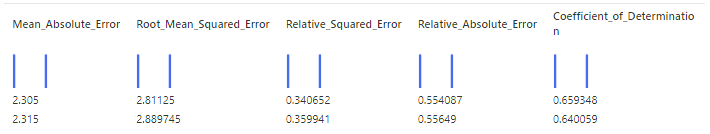
\includegraphics[height=30mm,scale=0.5]{./appendices/msg_ngram_decision-forest-reg_lewd2unanom.png}
    \caption{Message with N-Gram feature extraction
    using unconventional training method in phase 1,
        Decision forest regression in phase 2,
        compared to method without anomaly values.
        \label{fig:msg_ngram_decision-forest-reg_lewd2unanom}}
\end{figure}

\begin{figure}[htb]
    \centering
    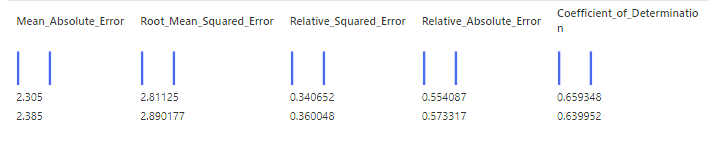
\includegraphics[height=30mm,scale=0.5]{./appendices/msg_ngram_decision-forest-reg_proper2unanom.png}
    \caption{Message with N-Gram feature extraction
    using proper training method in phase 1,
        Decision forest regression in phase 2,
        compared to method without anomaly values.
        \label{fig:msg_ngram_decision-forest-reg_proper2unanom}}
\end{figure}

\begin{figure}[htb]
    \centering
    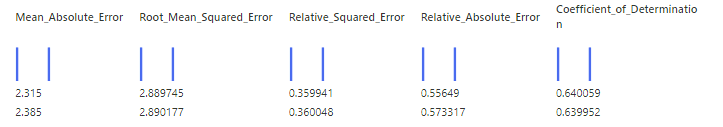
\includegraphics[height=30mm,scale=0.5]{./appendices/msg_ngram_decision-forest-reg_lewd2proper.png}
    \caption{Message with N-Gram feature extraction
    using Decision forest regression in phase 2,
        comparing unconventional training to proper training.
        \label{fig:msg_ngram_decision-forest-reg_lewd2proper}}
\end{figure}



\clearpage

\subsubsection*{Anomaly detection with pure textual data}

\begin{figure}[htb]
    \centering
    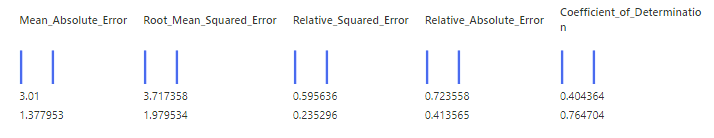
\includegraphics[height=30mm,scale=0.5]{./appendices/msg_pure_decision-forest-reg_lewd2unanom.png}
    \caption{Message fed pure to ADA-component,
    using unconventional training method in phase 1,
        Decision forest regression in phase 2,
        compared to method without anomaly values.
        \label{fig:msg_pure_decision-forest-reg_lewd2unanom}}
\end{figure}

\begin{figure}[htb]
    \centering
    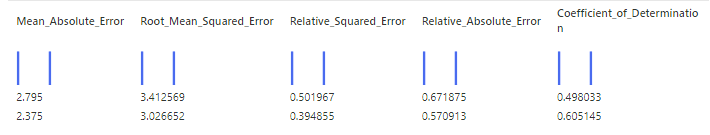
\includegraphics[height=30mm,scale=0.5]{./appendices/msg_pure_decision-forest-reg_proper2unanom.png}
    \caption{Message fed pure to ADA-component,
        using proper training method in phase 1,
        Decision forest regression in phase 2,
        compared to method without anomaly values.
        \label{fig:msg_pure_decision-forest-reg_proper2unanom}}
\end{figure}



\begin{figure}[htb]
    \centering
    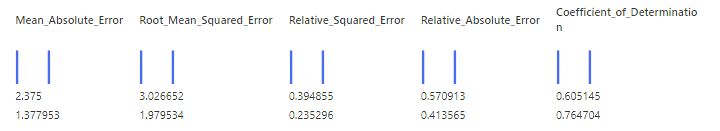
\includegraphics[height=30mm,scale=0.5]{./appendices/msg_pure_decision-forest-reg_lewd2proper.png}
    \caption{Message fed pure to ADA-component,
    using Decision forest regression in phase 2,
        comparing unconventional training to proper training.
        \label{fig:msg_pure_decision-forest-reg_lewd2proper}}
\end{figure}

\clearpage